
\documentclass[a4paper,8pt]{article}
\usepackage{graphicx}
\usepackage[margin=0.5in,top=0.5in,bottom=0.5in,left=0.75in]{geometry}
\usepackage{fancyhdr} % for custom headers and footers
\pagestyle{fancy} % set page style to fancy
\renewcommand{\headrulewidth}{0pt}
\fancyhf{} % clear default header and footer
\fancyfoot[C]{\thepage} % set center of footer to be the page number
\usepackage{float}
\begin{document}

        \section{Neighbourhood Operation}
        \begin{verbatim}
        import sys


input_file = sys.argv[1]
output_file = sys.argv[2]

# Read the input image file line by line
with open(input_file, 'r') as f:
    lines = f.readlines()

# Extract the image dimensions and pixel values
assert lines[0].startswith('P2')
width, height = map(int, lines[1].split())
max_value = int(lines[2])
pixels = [list(map(int, line.split())) for line in lines[3:]]

# Define the size of the neighborhood window (m x n)
m = 3  # number of rows in the neighborhood window
n = 3  # number of columns in the neighborhood window

# Define the Sxy set of pixel coordinates to use for the operation
Sxy = [(i, j) for i in range(-m//2, m//2+1) for j in range(-n//2, n//2+1)]

# Apply the neighborhood operation to each pixel in the input image
new_pixels = []
for y in range(height):
    new_row = []
    for x in range(width):
        # Extract the neighborhood window centered at (x, y)
        neighborhood = [(x + i, y + j) for i, j in Sxy if 0 <= x+i < width and 0 <= y+j < height]
        # Compute the average pixel value using the formula
        avg_value = sum(pixels[j][i] for i, j in neighborhood) / (m * n)
        new_row.append(int(avg_value))
    new_pixels.append(new_row)

# Write the processed image to the output file
with open(output_file, 'w') as f:
    f.write('P2\n')
    f.write(f'{width} {height}\n')
    f.write(f'{max_value}\n')
    for row in new_pixels:
        f.write(' '.join(str(p) for p in row))
        f.write('\n')


        \end{verbatim}
        
        \begin{figure}[H]
        \centering
        \begin{minipage}{0.4\linewidth}
        \centering
        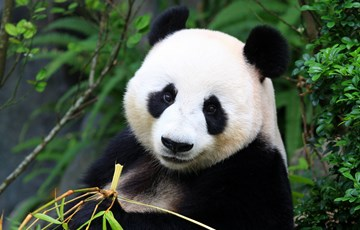
\includegraphics[width=\linewidth]{output/input1.jpg}
        \caption{Input}
        \end{minipage}
        \hfill
        \begin{minipage}{0.4\linewidth}
        \centering
        \includegraphics[width=\linewidth]{output/Neighbourhood Operation_output.png}
        \caption{Output}
        \end{minipage}
        \end{figure}
        \clearpage
        
        \section{Histogram Equalization}
        \begin{verbatim}
        import sys

input_file = sys.argv[1]
output_file = sys.argv[2]

with open(input_file, 'r') as picture:
    element = picture.readlines()

frequency = {}
pdf = {}
cdf = {}
mapping = {}
for i in range(256):
    frequency[f'{i}'] = 0
    pdf[f'{i}'] = 0
    cdf[f'{i}'] = 0
    mapping[f'{i}'] = 0
    
for i in range(4, len(element)-4):
    frequency[element[i].replace('\n', '')] += 1

for i in range(256):
    pdf[f'{i}'] = round(frequency[f'{i}'] / (len(element)-4), 3)

cdf['0'] = pdf['0']
for i in range(1, 256):
    cdf[f'{i}'] = cdf[f'{i-1}'] + pdf[f'{i}']

for i in range(256):
    mapping[f'{i}'] = round(255 * cdf[f'{i}'])

with open(output_file, 'w') as out:
    for i in range(4, len(element)-4):
        element[i] = str(mapping[element[i].replace('\n', '')]) + '\n'
    out.writelines(element)


        \end{verbatim}
        
        \begin{figure}[H]
        \centering
        \begin{minipage}{0.4\linewidth}
        \centering
        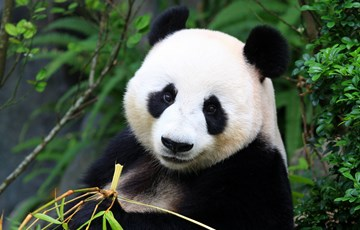
\includegraphics[width=\linewidth]{output/input1.jpg}
        \caption{Input}
        \end{minipage}
        \hfill
        \begin{minipage}{0.4\linewidth}
        \centering
        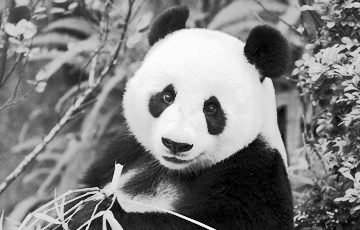
\includegraphics[width=\linewidth]{output/Histogram Equalization_output.png}
        \caption{Output}
        \end{minipage}
        \end{figure}
        \clearpage
        
        \section{Log Transformation}
        \begin{verbatim}
        from math import log10
import sys


input_file = sys.argv[1]
output_file = sys.argv[2]
input_image = np.loadtxt(input_file, skiprows=3)


with open(input_file, 'r') as picture:
    element = picture.readlines()

with open(output_file, 'w') as out:
    for i in range(len(element) - 4):
        element[i+4] = str( int(104 * log10(1 + int(element[i+4].replace('\n', ''))))) + '\n'
    out.writelines(element)

        \end{verbatim}
        
        \begin{figure}[H]
        \centering
        \begin{minipage}{0.4\linewidth}
        \centering
        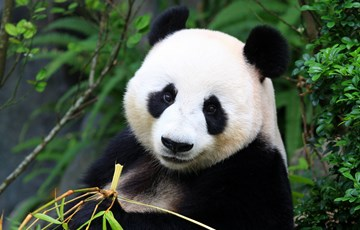
\includegraphics[width=\linewidth]{output/input1.jpg}
        \caption{Input}
        \end{minipage}
        \hfill
        \begin{minipage}{0.4\linewidth}
        \centering
        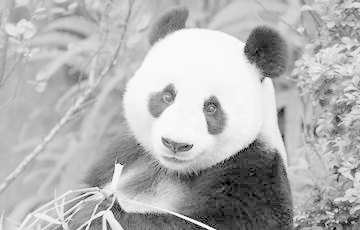
\includegraphics[width=\linewidth]{output/Log Transformation_output.png}
        \caption{Output}
        \end{minipage}
        \end{figure}
        \clearpage
        
        \section{Power Law Transformation}
        \begin{verbatim}
        import sys
from math import pow


input_file = sys.argv[1]
output_file = sys.argv[2]
gamma = 2
C = 5

with open(input_file, 'r') as picture:
    element = picture.readlines()

with open(output_file, 'w') as out:
    for i in range(len(element) - 4):
        pix = int(C * pow(int(element[i+4].replace('\n', '')), gamma))
        if pix > 255:
            element[i+4] = '255\n'
        elif pix < 0:
            element[i+4] = '0\n'
        else:
            element[i+4] = str(pix) + '\n'
    out.writelines(element)


        \end{verbatim}
        
        \begin{figure}[H]
        \centering
        \begin{minipage}{0.4\linewidth}
        \centering
        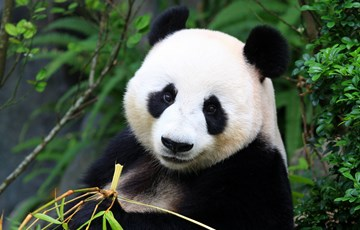
\includegraphics[width=\linewidth]{output/input1.jpg}
        \caption{Input}
        \end{minipage}
        \hfill
        \begin{minipage}{0.4\linewidth}
        \centering
        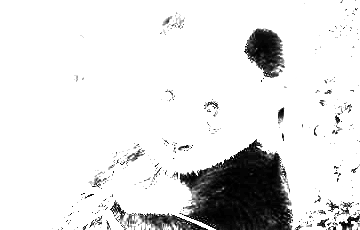
\includegraphics[width=\linewidth]{output/Power Law Transformation_output.png}
        \caption{Output}
        \end{minipage}
        \end{figure}
        \clearpage
        
        \section{Negative Transformation}
        \begin{verbatim}
        import sys

if len(sys.argv) < 3:
    print("Usage: python myscript.py input.pgm output.pgm")
    sys.exit(1)

input_file = sys.argv[1]
output_file = sys.argv[2]

with open(input_file, 'r') as picture:
    element = picture.readlines()

with open(output_file, 'w') as out:
    for i in range(len(element) - 4):
        element[i+4] = str(255 - int(element[i+4].replace('\n', ''))) + '\n'
    out.writelines(element)


        \end{verbatim}
        
        \begin{figure}[H]
        \centering
        \begin{minipage}{0.4\linewidth}
        \centering
        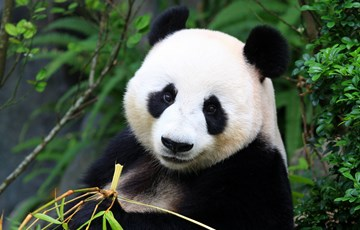
\includegraphics[width=\linewidth]{output/input1.jpg}
        \caption{Input}
        \end{minipage}
        \hfill
        \begin{minipage}{0.4\linewidth}
        \centering
        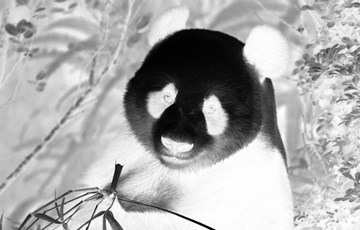
\includegraphics[width=\linewidth]{output/Negative Transformation_output.png}
        \caption{Output}
        \end{minipage}
        \end{figure}
        \clearpage
        
        \section{Noise Matrix}
        \begin{verbatim}
        import numpy as np
import random
import sys

    
input_file = sys.argv[1]
input_image = np.loadtxt(input_file, skiprows=3)

# Generate 10 noisy images
noisy_images = []
for i in range(10):
    # Generate uncorrelated noise matrix
    noise_matrix = np.zeros_like(input_image)
    for x in range(input_image.shape[0]):
        for y in range(input_image.shape[1]):
            noise_matrix[x][y] = random.uniform(-1, 1)
    
    # Add noise to input image
    noisy_image = input_image + noise_matrix
    noisy_images.append(noisy_image)

# Apply averaging to resolve noise
averaged_image = np.zeros_like(input_image)
for x in range(input_image.shape[0]):
    for y in range(input_image.shape[1]):
        pixel_sum = 0
        for noisy_image in noisy_images:
            pixel_sum += noisy_image[x][y]
        averaged_image[x][y] = pixel_sum / 10

# Write averaged image to file
output_file = input_file[:-4] + "_averaged.pgm"
with open(output_file, "w") as f:
    # Write header
    f.write("P2\n")
    f.write("# Averaged image\n")
    f.write("{} {}\n".format(averaged_image.shape[1], averaged_image.shape[0]))
    f.write("255\n")

    # Write pixel values
    for x in range(averaged_image.shape[0]):
        for y in range(averaged_image.shape[1]):
            f.write(str(int(averaged_image[x][y])) + " ")
        f.write("\n")



        \end{verbatim}
        
        \begin{figure}[H]
        \centering
        \begin{minipage}{0.4\linewidth}
        \centering
        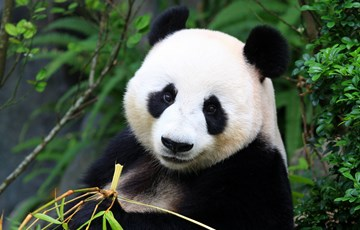
\includegraphics[width=\linewidth]{output/input1.jpg}
        \caption{Input}
        \end{minipage}
        \hfill
        \begin{minipage}{0.4\linewidth}
        \centering
        \includegraphics[width=\linewidth]{output/Noise Matrix_output.png}
        \caption{Output}
        \end{minipage}
        \end{figure}
        \clearpage
        
\end{document}
